\chapter{Introduzione al Corso}

\begin{itemize}
	\item{\textbf{Logica Booleana}}
	\item{\textbf{Aritmetica Binaria}}
	\item{\textbf{Reti Logiche}}
	\item{\textbf{Microarchitettura e Assembler ARM v7 e v8}}
	\item{\textbf{Gestione della memoria}}
	\item{\textbf{I/O}}
\end{itemize}

\paragraph{Strumenti Software}
A differenza degli A.A passati utilizzeremo Verilog e Assembler ARM.
Utilizzeremo \textbf{iverilog} come compilatore Verilog e \textbf{gtkwave} come tool grafico. Un ambiente di sviluppo Verilog completo che vedremo è \textbf{Quartus}.
Per la seconda parte del corso, Assembler ARM, useremo la \textbf{toolchain GNU}, in particolare:


\subparagraph{Se non hai una macchina ARM:}
\begin{itemize}
	\item{cross-compiler per compilare}
	\item{QEMU per una macchina virtuale ARM}
	\item{gdb per debugging}
\end{itemize}

\subparagraph{Se hai una macchina ARM come un Raspberry Pi:}
\begin{itemize}
	\item{Toolchain GNU per compilare}
	\item{Cavo Ethernet}
	\item{Server SSH sulla macchina ARM per accesso remoto}
\end{itemize}

\paragraph{Storia degli Elaboratori}

\begin{figure}
	\centering
	\caption{Sinclair ZX80}
	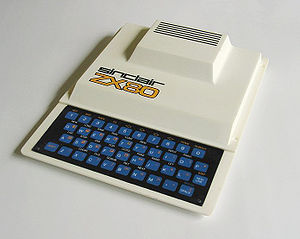
\includegraphics[width=0.5\textwidth]{ZX80}
\end{figure}

Nei corsi di Architettura degli Elaboratori negli anni 80 i processori studiati erano: il 6502 (8 bit, processore del computer Apple II, noto per essere stato costruito nel garage di Steve Jobs e Wozniak), Z80, processore a 16 bit del famoso computer ZX80 e l'Intel 8088. Tali processori raggiungevano al massimo una velocità di clock (detto molto a grandi linee, operazioni al secondo) dell'ordine di meno di una decina di MHz (Mega Hertz, milioni). I processori odierni raggiungono
cicli di clock sull'ordine dei GHz (Giga Hertz, miliardi). Nel corso degli anni fino ad oggi, l'evoluzione dei processori ha seguito la \textbf{legge di Moore}. La "legge" spiega che ogni 18 mesi la potenza dei processori in commercio raddoppia, perché la densità dei transistor contenuti all'interno aumenta. Negli ultimi decenni abbiamo  miglioramenti architetturali come super pipeline e super scalari, ciò ha permesso di introdurre processori \textbf{multicore}, ovvero che contengono più "nuclei" interni (detti core) che elaborano le istruzioni dei processi in esecuzione in parallelo.
Ad oggi il numero di core in uno smartphone raggiunge anche gli 8 core, mentre in processori per server sono stati raggiunti numeri di core anche intorno ai 64. I processori odierni utilizzano core a 64 bit, con architettura X86\_64 per Desktop o ARM per dispositivi mobili.
Un componente fondamentale dell'evoluzione degli elaboratori è stato anche lo sviluppo dei processori grafici (GPU) con i quali ad oggi è possibile riprodurre grafica su schermo, ambienti tridimensionali molto complessi (videogiochi) o sfruttare la loro capacità di parallelizzazione per l'uso di reti neurali nell'intelligenza artificiale.

Osserveremo i calcolatori a diversi livelli di \textbf{astrazione}

I livelli di astrazione sono:
\begin{itemize}
	\item Applicazioni utente
	\item Sistema Operativo
	\item Architettura (ASM, ad es. x86 o ARM)
	\item Microarchitettura
	\item Logica
	\item Circuiti digitali
	\item Device
	\item Fisica
\end{itemize}

Ogni livello si appoggia sul livello inferiore, ovvero è costruito sui componenti offerti dal livello inferiore. Dei principi fondamentali sono: \textbf{gerarchi, modularità e regolarità}

La modularità è fondamentale per avere moduli organizzati gerarchicamente, autonomi ed indipendenti.

\paragraph{Set di Istruzioni}

Distinguiamo due set di istruzioni dei processori, \textbf{CISC} e \textbf{RISC}. Gli acronimi sono rispettivamente \textbf{Complex Instruction Set Computer} e \textbf{Reduced Instruction Set Computer}, RISC contiene i processori ARM, che studieremo in dettaglio, mentre CISC comprende i processori più comuni nei desktop (X86 e X86\_64)


